\documentclass[a4paper,11pt]{article}
\usepackage{graphicx}
\usepackage{enumerate}
\usepackage[usenames, dvipsnames]{color}
\usepackage[margin=1.25in]{geometry}
\usepackage{hyperref}

\usepackage{setspace}
\doublespacing

\begin{document}

\begin{flushright}

\vspace{1.1cm}

{\bf\Huge Correlating Hubble Telescope Dark-Rates with Solar Activity}

\rule{0.25\linewidth}{0.5pt}

\vspace{0.5cm}
%Put Authors
Justin Ely
\linebreak
%Put Author's affiliations
\footnotesize{605.462 Data Visualization \\}
% Date here below
08 May, 2017
\end{flushright}

\noindent\rule{\linewidth}{1.0pt}

%%%%%%%%%%%%%%%%%%%%%%%%%%%%%%%%%%%%%%%%%%%%%%%%%%%%%%%%%%

\section{Abstract}
In this paper we use custom data processing and a new exploratory website to deeper understand the 
relationship between increased darkrates in data from the Cosmic Origins Spectrograph (COS) and solar activity.  
Through this investigation we see that the observed fluctuations cannot be solely due to increased solar output
during certain periods of time, and that another factor must be in play.  By viewing the data in new ways, we find 
that increased darkrates on the COS far-ultraviolet (FUV) detectors depend both on solar activity and orbital position relative to the sub-solar point.   

\section{Introduction}
Electronic detectors, whether scientific or consumer grade, are subject to various forms of noise.  One common 
noise source, referred to as a darkrate,  is the accumulation of photons even when the main shutter is closed.  This is
generally a small source of noise; often dwarfed by the actual signal and corrected with minimal processing 
through well-understood processes.  However, on highly tuned scientific instruments, like the 
Hubble Space Telescope (HST), even the darkrate can be a difficult problem that needs to be addressed.

HST, in orbit since 1990, has had a variety of instruments with which to perform scientific observations.  Over the course of
their lifetime, many degrade and fail only to be subsequently replaced by astronauts.  The COS instrument is a recent addition,
having been installed in 2009.  This instrument uses a specialized detector called a cross delay line (XDL) 
which is optimized to detect light in the ultra-violet (UV) band \cite{fox}. The XDL is designed for 
observing extremely faint objects, which makes accounting for every noise source very important.  Though for
many of the brighter possible targets the COS darkrate can be safely ignored, for those on the fainter side it can 
be a significant hurdle.  This makes understanding the behavior of the darkrate very important to many researchers.

The Hubble Space Telescope (HST) occupies a region of space called low-earth orbit
which extends from 160 and 2000 kilometers above the surface of the Earth \cite{leo}.   At $\sim$547 km,  HST 
can have significant interaction with the atmosphere and magnetic fields surrounding Earth \cite{hst}.  The telescope assembly
 itself experiences drag from the upper exosphere, which causes orbital decay and will eventually cause HST to 
 re-enter the atmosphere.  The individual instruments also experience the LEO environment in different ways.  
 In particular, the COS instrument is sensitive to contamination from energetic particles from Earth's magnetic fields,
 the sun, and even distant extra-galactic objects \cite{fox} \cite{norton}.

One significant force in the environment of LEO is the solar cycle.  This is the periodic ebb and flow of the sun's 
output over time.  The typical period is between 10 and 12 years and includes fluctuations in sunspot
 number and solar flar frequency. \cite{mercedes}.  The varying solar output during the solar cycle causes changes
 in the atmospheric scale height, density of charged particles in the radiation belts, and an increased solar wind
 throughout the solar system \cite{mercedes}.

\section{Background}
The staff at the Space Telescope Science Institute (STScI) have been monitoring the COS 
dark rate since it's installation in 2009 \cite{fox}.  Approximately bi-weekly, the instrument has taken a set of 
observations with the external shutter closed in order to get an accurate sample of the darkrate.  These 
observations were then used to create and disseminate confidence intervals to the astronomical community 
for planning and data reduction purposes.  Through repeated measurement and long-term analysis, they suggest a correlation of
the darkrate with the intensity of the solar cycle output.  Their results from their monitoring are shown in Figure 1.    

The National Oceanic and Atmospheric Administration (NOAA) maintains a number of on-going 
efforts to monitor the sun and solar environment.  One common metric to measure solar output is the F10.7 index \cite{norton}.  This index measures the solar output at 10.7 cm, in the Radio band,
and at 70 years is one of the longest on-going records of solar activity.  The F10.7 index has been shown to track well with UV solar emissions that interact with earth's stratosphere \cite{norton}.  Since this tracks well with UV, the band that the COS instrument is sensitive to, this makes it a useful index for the current investigation.

\begin{figure}[h!]
\caption{STScI produced analysis of the darkrate history of the COS FUV detectors \cite{fox}. The top plot shows 
measured darkrates, while the bottom plots shows the F10.7 index.  A loose correlation with the overall trend of the
solar output can be seen, wich significant devations.}
\centering
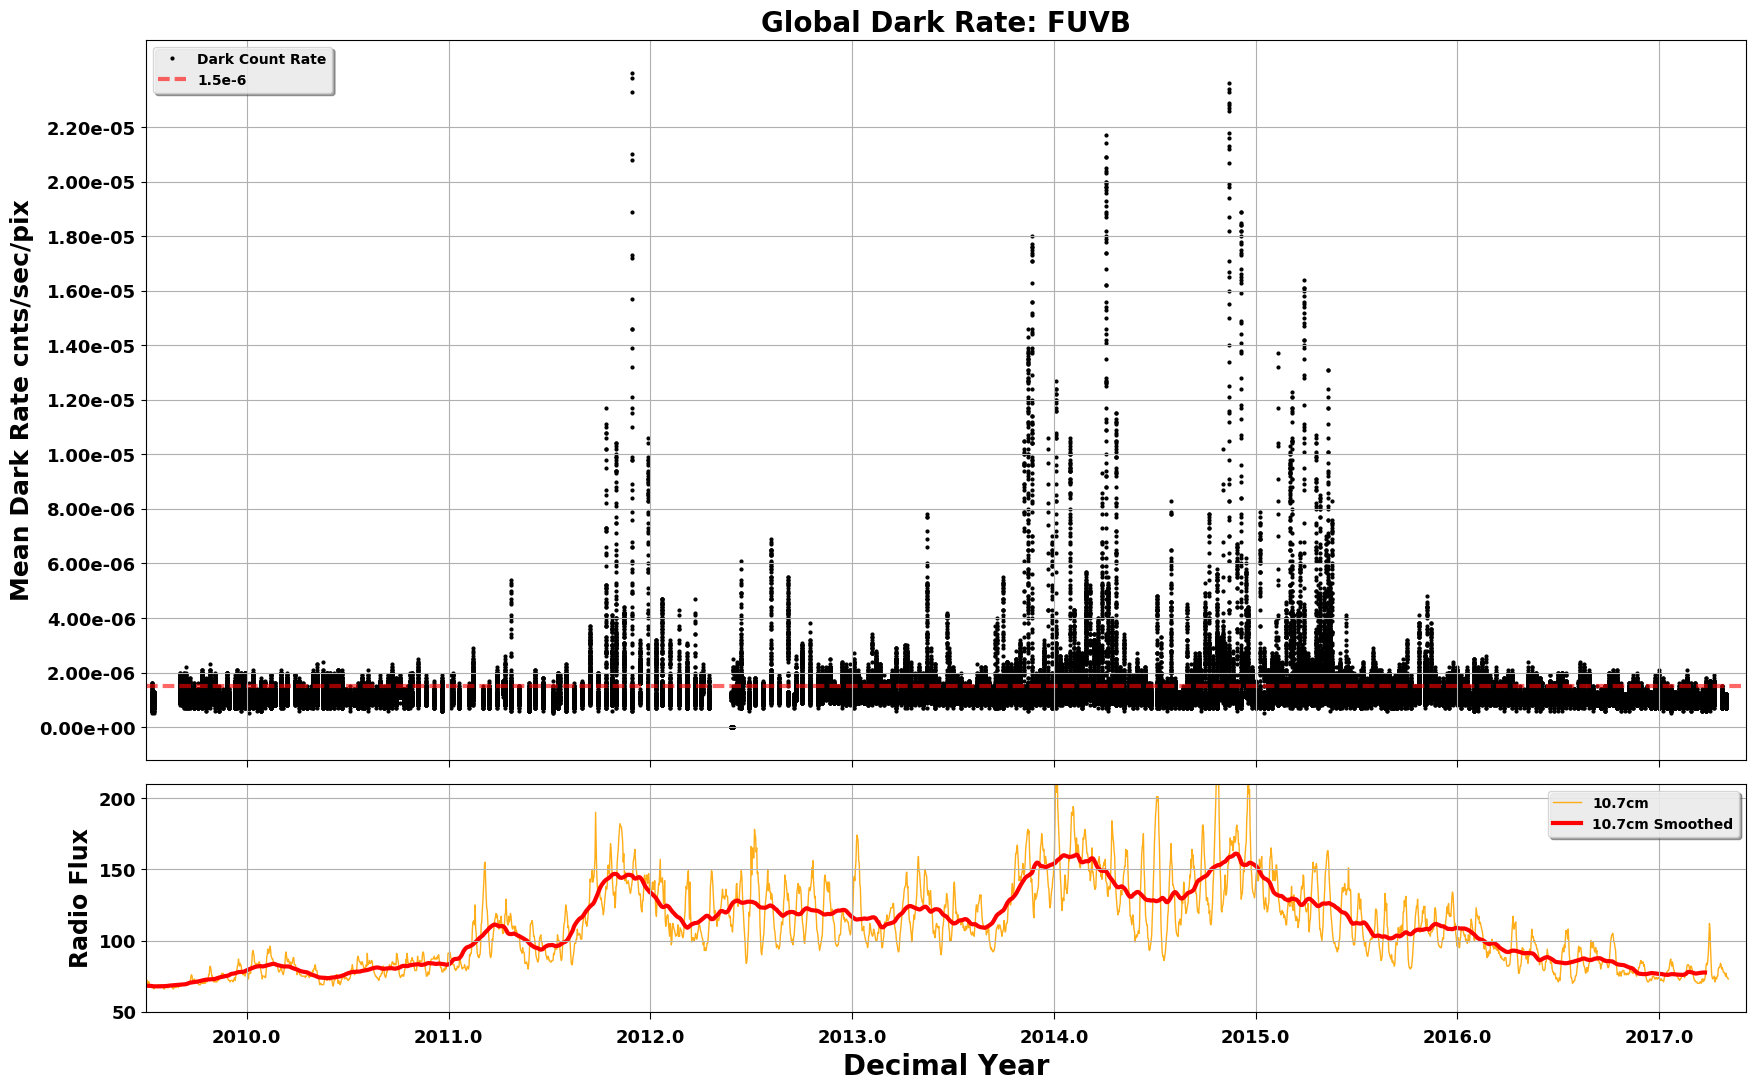
\includegraphics[width=.8\textwidth]{dark_vs_time_FUVB.png}
\end{figure}

The STScI data does seem to indicate a general correlation between high darkrates and solar cycle output.  Periods of 
high solar output, mostly between late 2013 to mid 2015, also correspond to times when the dark rate would 
periodically spike.  Periods of low solar activity, pre-2011 and post-2016, all show zero detected spikes.  However, the 
majority of the data appears to be centered on a low value even when solar output is high.  This indicates that the 
spikes are responding to something else as well.

One possible explanation of this behavior is that the spikes in observed darkrate come from a more direct interaction 
with solar radiation, rather than just the general increase in output.  We hypothesize that the spikes happen when solar output is high, and when HST passes near the point on the earth directly opposite the sun (the sub-solar point) and 
is bombarded with higher than usual radiation levels.

\section{Approach}
To tackle this question, we first needed to gather and process the required data. This
required all of the COS data taken with the shutter closed, as well as the F10.7 index data for the 
timeframe of the COS data. 

The COS instrument takes data frequently, but the vast majority of the observations are of
an astronomical object that is orders of magnitude above the darkrate and can often be 
intrinsically variable.  Fortunately, as mentioned before, the COS instrument team schedules observations with the 
external shutter closed every couple of weeks specifically to measure and track the darkrate.
These datasets were retrieved through the MAST portal at \href{https://archive.stsci.edu/hst/search.php}{https://archive.stsci.edu/hst/search.php}.  To get all the correct datasets, the form was  filled in as specified below.  This returned the 2426 dark datasets taken to date for the COS instrument.

\begin{enumerate}
	\item {\bf Target Name} set to "DARK".
	\item {\bf Resolver} set to "Don't Resolve".
	\item {\bf COS} box under {\bf Imagers} checked.
	\item {\bf Calibration} box under {\bf Observations} checked.
\end{enumerate}

After retrieval, the COS data need to be calibrated using a custom data processing pipeline.  Though
STScI provides standard calibration software for the community to use, it did not include a calculation
necessary to this investigation; namely the position of the sub-solar point during the observation.  The author 
forked the code for the standard calibration
pipeline, named CalCOS, and modified it to calculate and output the sub-solar point to each of the 
individual data products.  The location for the modified source code can be found in the Appendix.

Next, the F10.7 index data needed to be retrieved.  The data taken since 1994, 
measured daily, is kept in the NOAA public FTP site:
 \href{ftp://ftp.swpc.noaa.gov/pub/indices/old\_indices/}{ftp://ftp.swpc.noaa.gov/pub/indices/old\_indices/}.  A simple FTP of all 
 datasets ending in "\_DSD.txt" was sufficient to gather this data locally. These two data collections where then joined and output in JSON format. The location for the source code to perform data gathering and compilation can be found in the Appendix. 
 
The dataset was then uploaded to a custom web application
built to study this problem.  This website uses javascript and the D3 graphics library to create a set of interactive 
visualizations through which to study this dataset.  The dashboard consists of three main parts; the 
tool bar, the map graphic, and the scatterplot graphic.  The map showed the darkrate measurements plotted against
latitude and longitude, as well as the location of the sub-solar point.  The scatterplot showed the behavior of the 
darkrate and F10.7 index over time, similar to the STScI analysis done previously.  The available toolbar permitted the
manipulation of datapoint size, opacity, and the filtering of unwanted points based on detector, time, and darkrate.  An additional selector would move the map points from native latitude and longitude coordinates into a frame relative to the sub-solar point.  

During the exploration of the data and development of the website, we reduced the extent of the loaded dataset
to help the visualization process and completely filter out useless data.  The first of these reductions was in the 
sheer number of points loaded.  The native format of the COS data has a sampling on the order of milliseconds, 
but a millisecond sampling over the lifetime of the intsrument would be many billions of points.  Even reducing down 
to the $\sim$second timescale resulted in too many datasets for the visualizations to load and render 
enough.  A good balance of sampling and performance was found by binning the data to $\sim$600 seconds,
which yielded 4k individual points to render. 

Also removed from the sample was all data taken with the near-ultraviolet (NUV) detector.  A very quick exploration of the data from this detector
showed that its short and long-term behavior showed little resemblance to the FUV behavior.  Upon further 
investigation, this is due to long-term out-gassing of the instrument and the temperature
dependence of the darkrate which dominates over the influence of the solar cycle.  As these data no longer assisted 
in the investigation, they were removed from the visualization.

\section{Results}
The results of our investigation are summarized in Figures 2 through 6.  Though many other views were used 
and manipulated throughout the exploration phase, these summarize the key views.

Figures 2 and 3 show the world graphic with the unfiltered dataset overplotted.  While Figure 2 displays the
dataset in the native latitude and longitude coordinates, Figure 3 shows the same points relative to the 
sub-solar point.  Any possible relation is obscured by the enormity of the dataset, and filtering and shrinking
pointsizes aren't enough to see the clear picture. 

From Figure 4, we see that the large spikes in dark rate are all above $\sim$4.5e-6 (counts/second/pixel).  
Since we're interested in correlating these deviant points, filtering the data to exclude points with lower 
darkrates than this threshold yielded Figures 4 and 5.  First in latitude/longitude, and then relative to the
sub-solar point, the difference is striking.  All of the high deviant points were observed to group slightly east of the sub-solar
point.  

\begin{figure}[!tbp]
  \centering
  \begin{minipage}[b]{0.4\textwidth}
    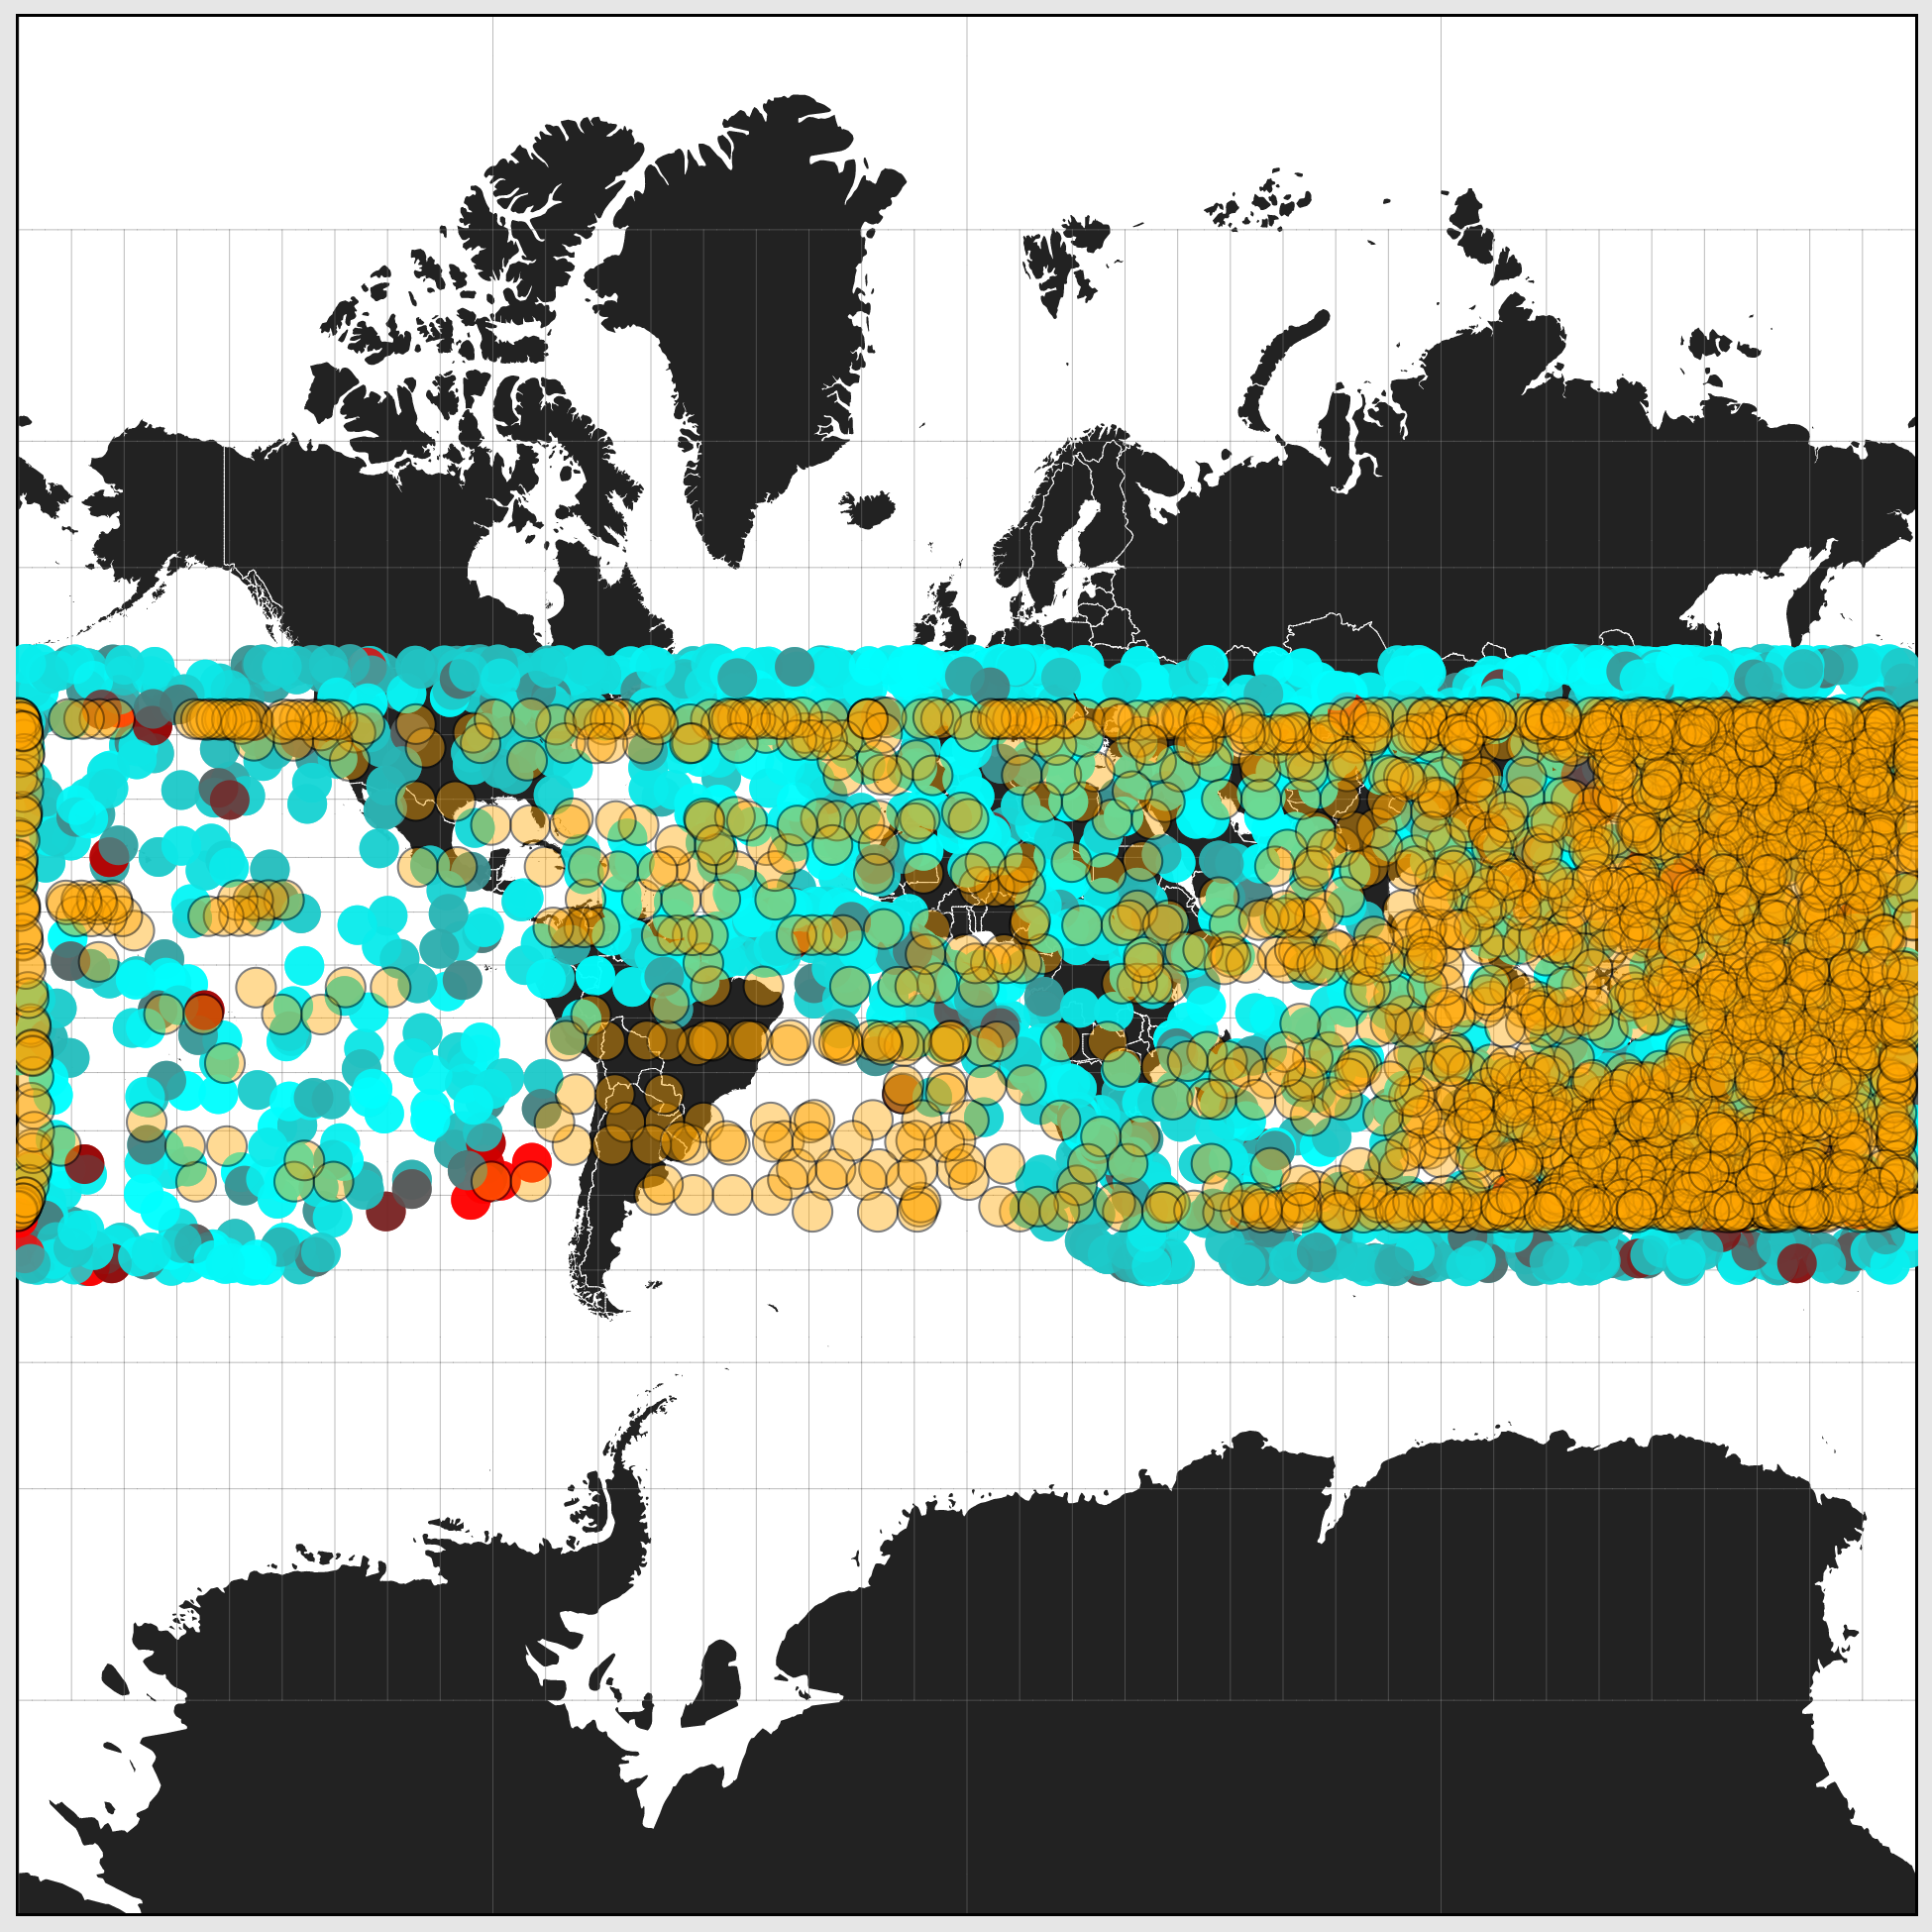
\includegraphics[width=\textwidth]{raw-lat-long.png}
    \caption{Map graphic showing all datapoints in latitude/longitude coordinates.  Sub-solar points are yellow with 
    black edges.  Note the gap in orbital coverage in the area of the South Atlantic Anomoly (SAA) \cite{norman} where
    magnetic field lines converge.  The COS detectors are shut off in this area to prevent damage. }
  \end{minipage}
  \hfill
  \begin{minipage}[b]{0.4\textwidth}
    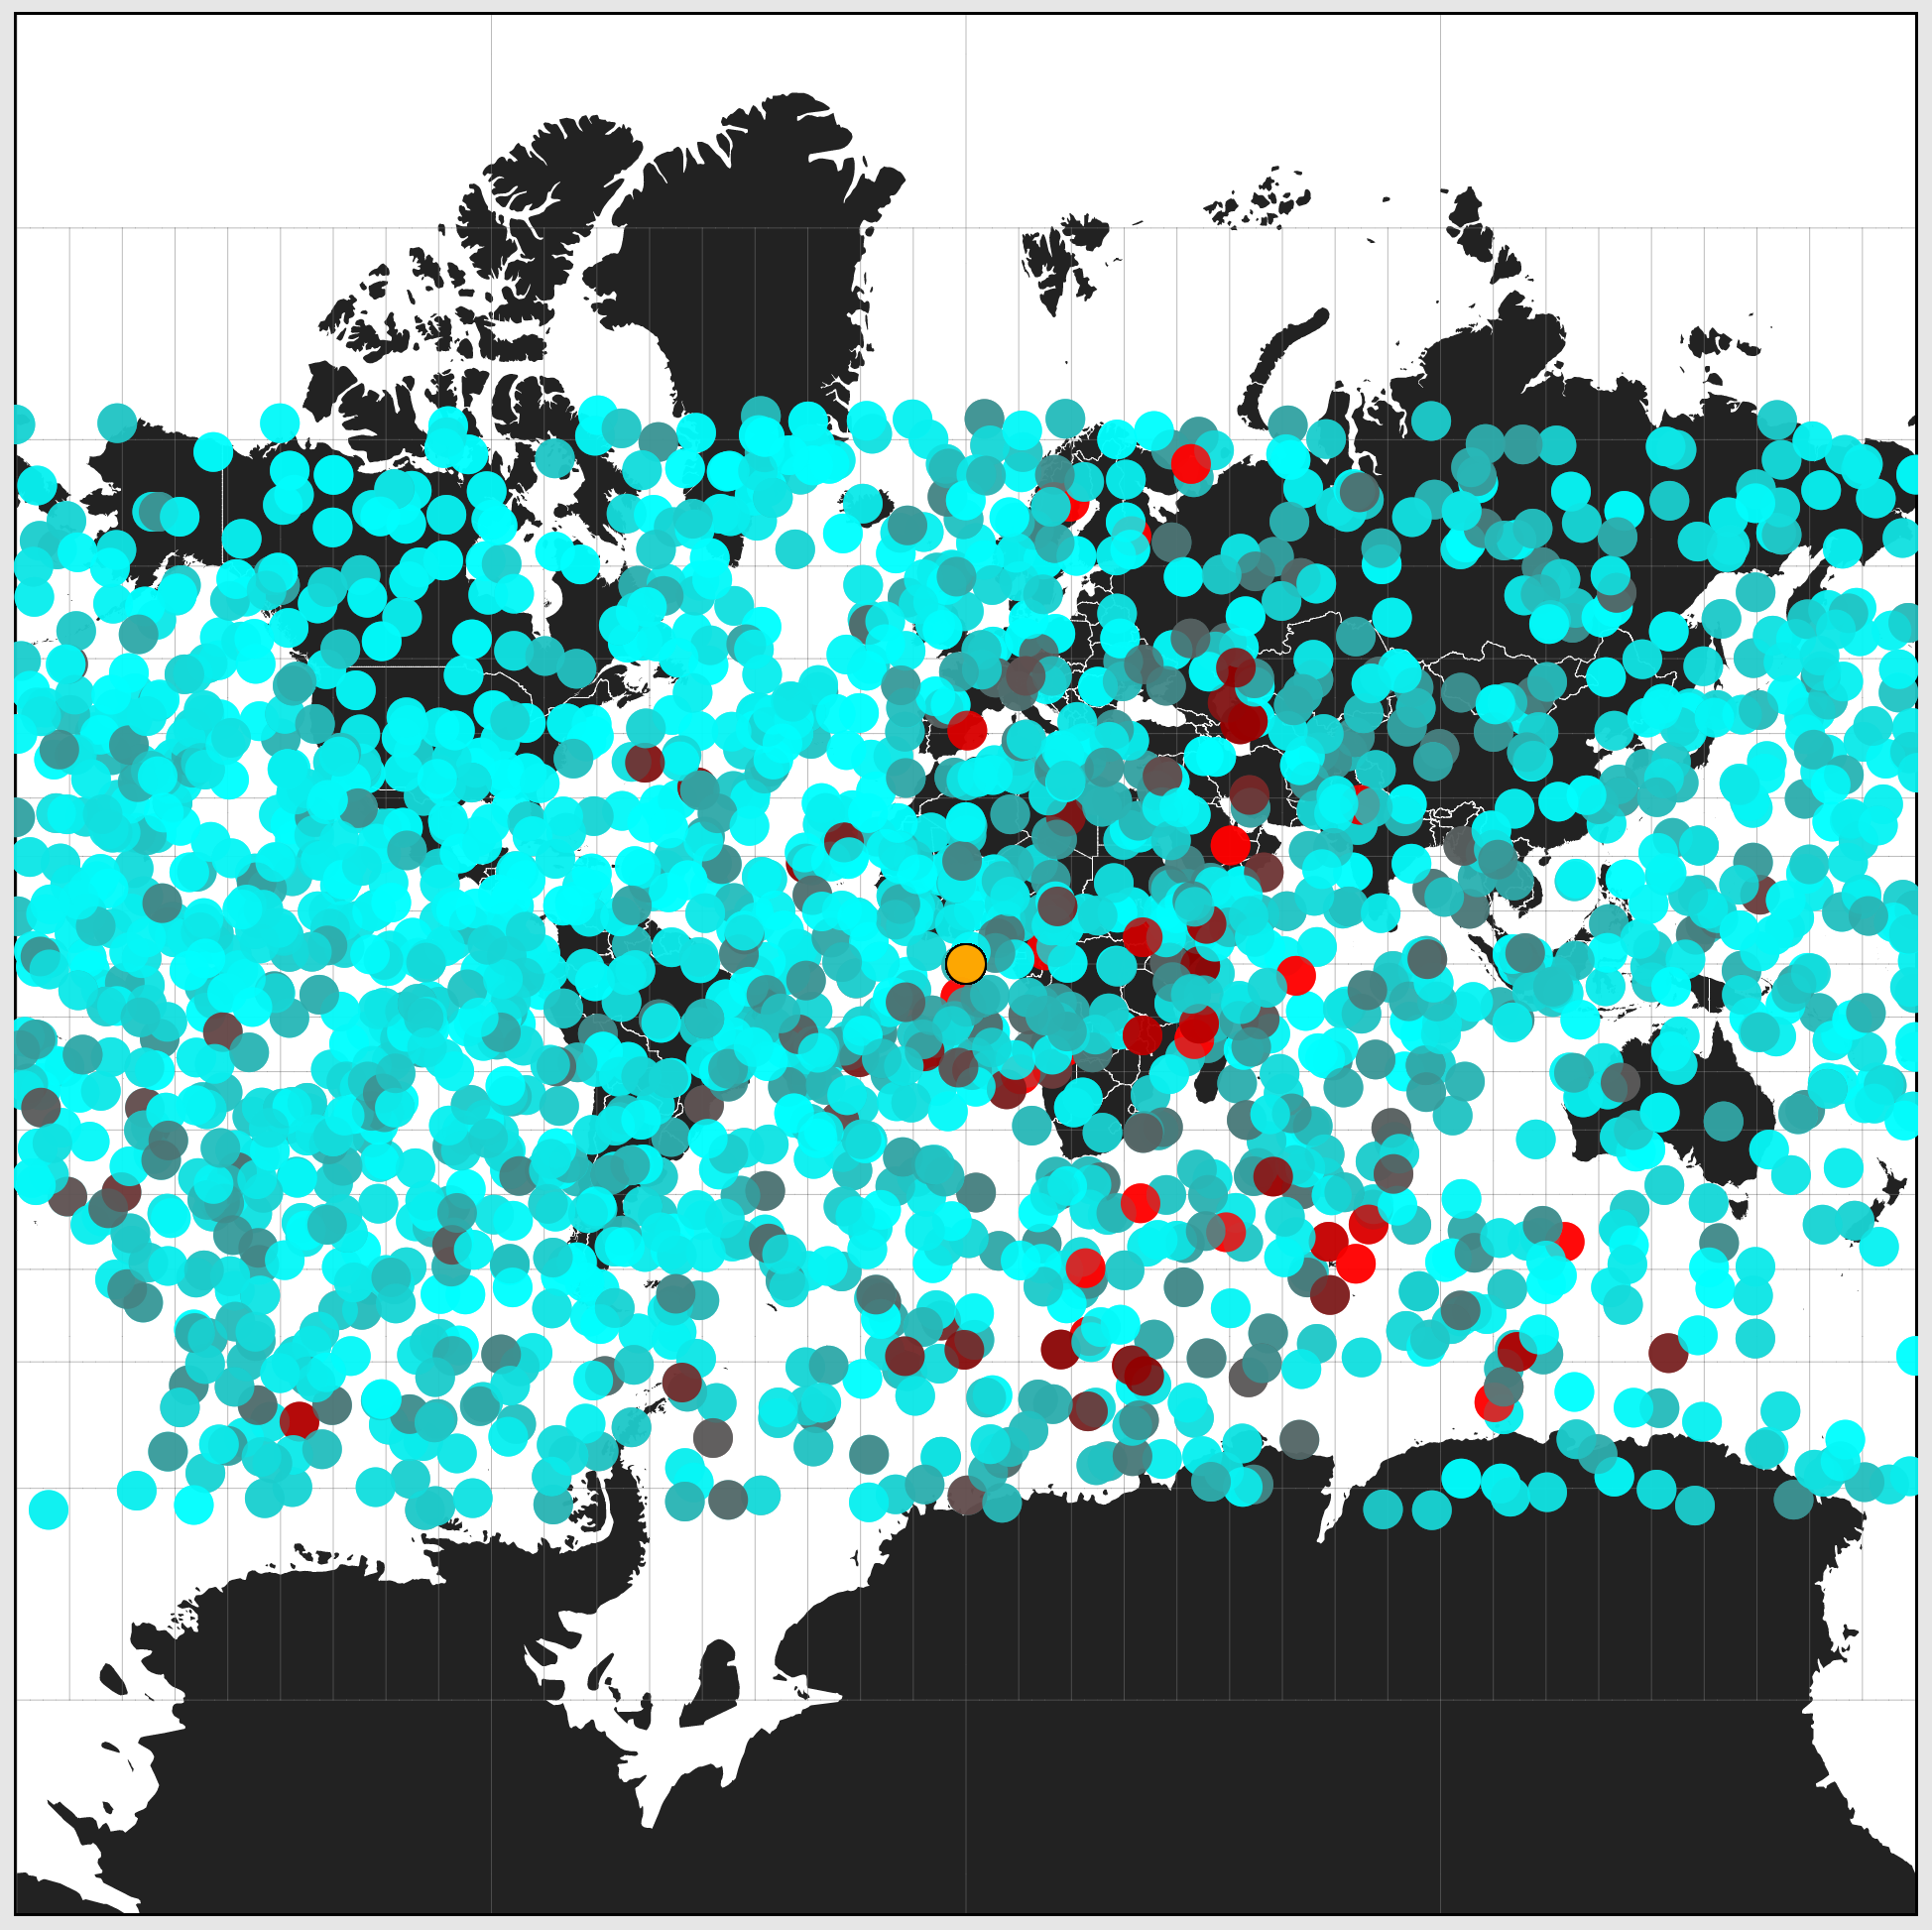
\includegraphics[width=\textwidth]{raw-sub-solar.png}
    \caption{Map graphic showing all datapoints in coordinates relative to the sub-solar point (located at the center, or
    (0, 0) in lat/long.  Any relation to the map background holds no relevance in this frame.  Similarly, the SAA cannot 
    be seen in this view due to the scrambling of positions.  }
  \end{minipage}
\end{figure}

\begin{figure}[h!]
\caption{Darkrate and F10.7 index plotted against time for all available datapoints.  Periods of high solar output 
 loosely correlate with high observed darkrates.}
\centering
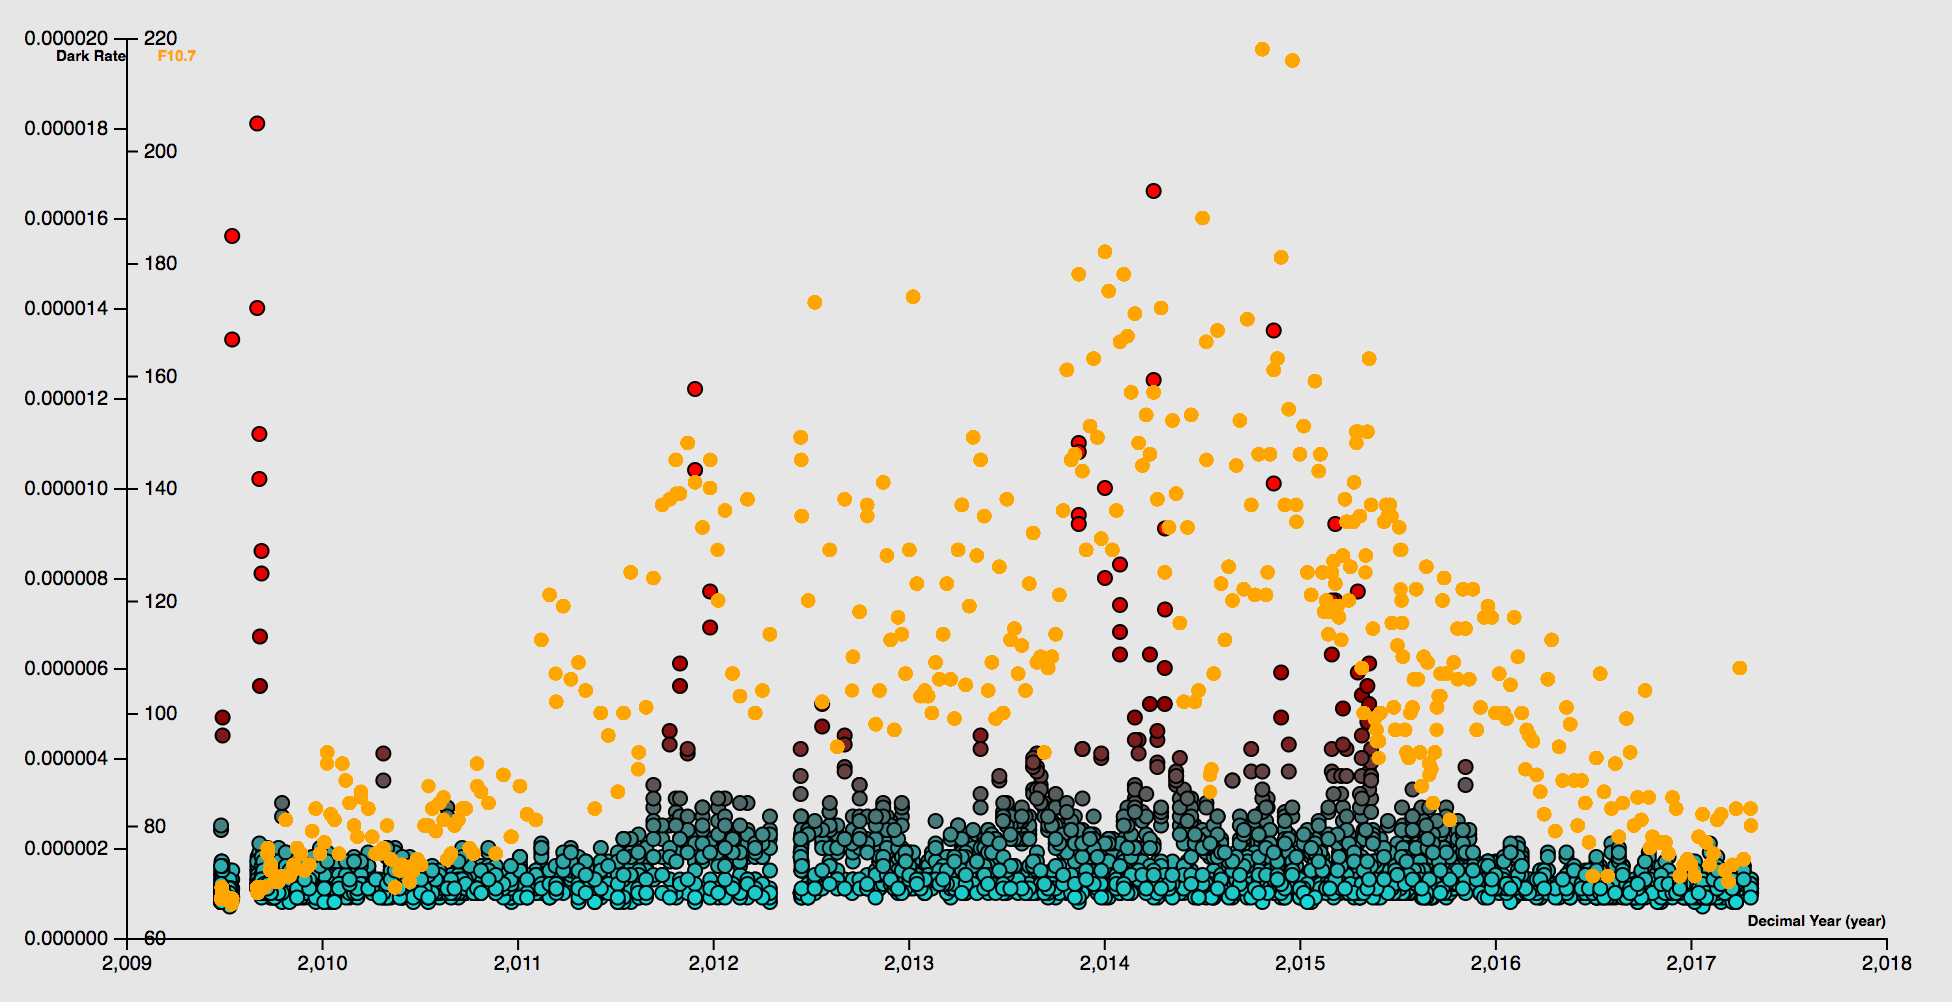
\includegraphics[width=.6\textwidth]{dark-time.png}
\end{figure}

\begin{figure}[!tbp]
  \centering
  \begin{minipage}[b]{0.4\textwidth}
    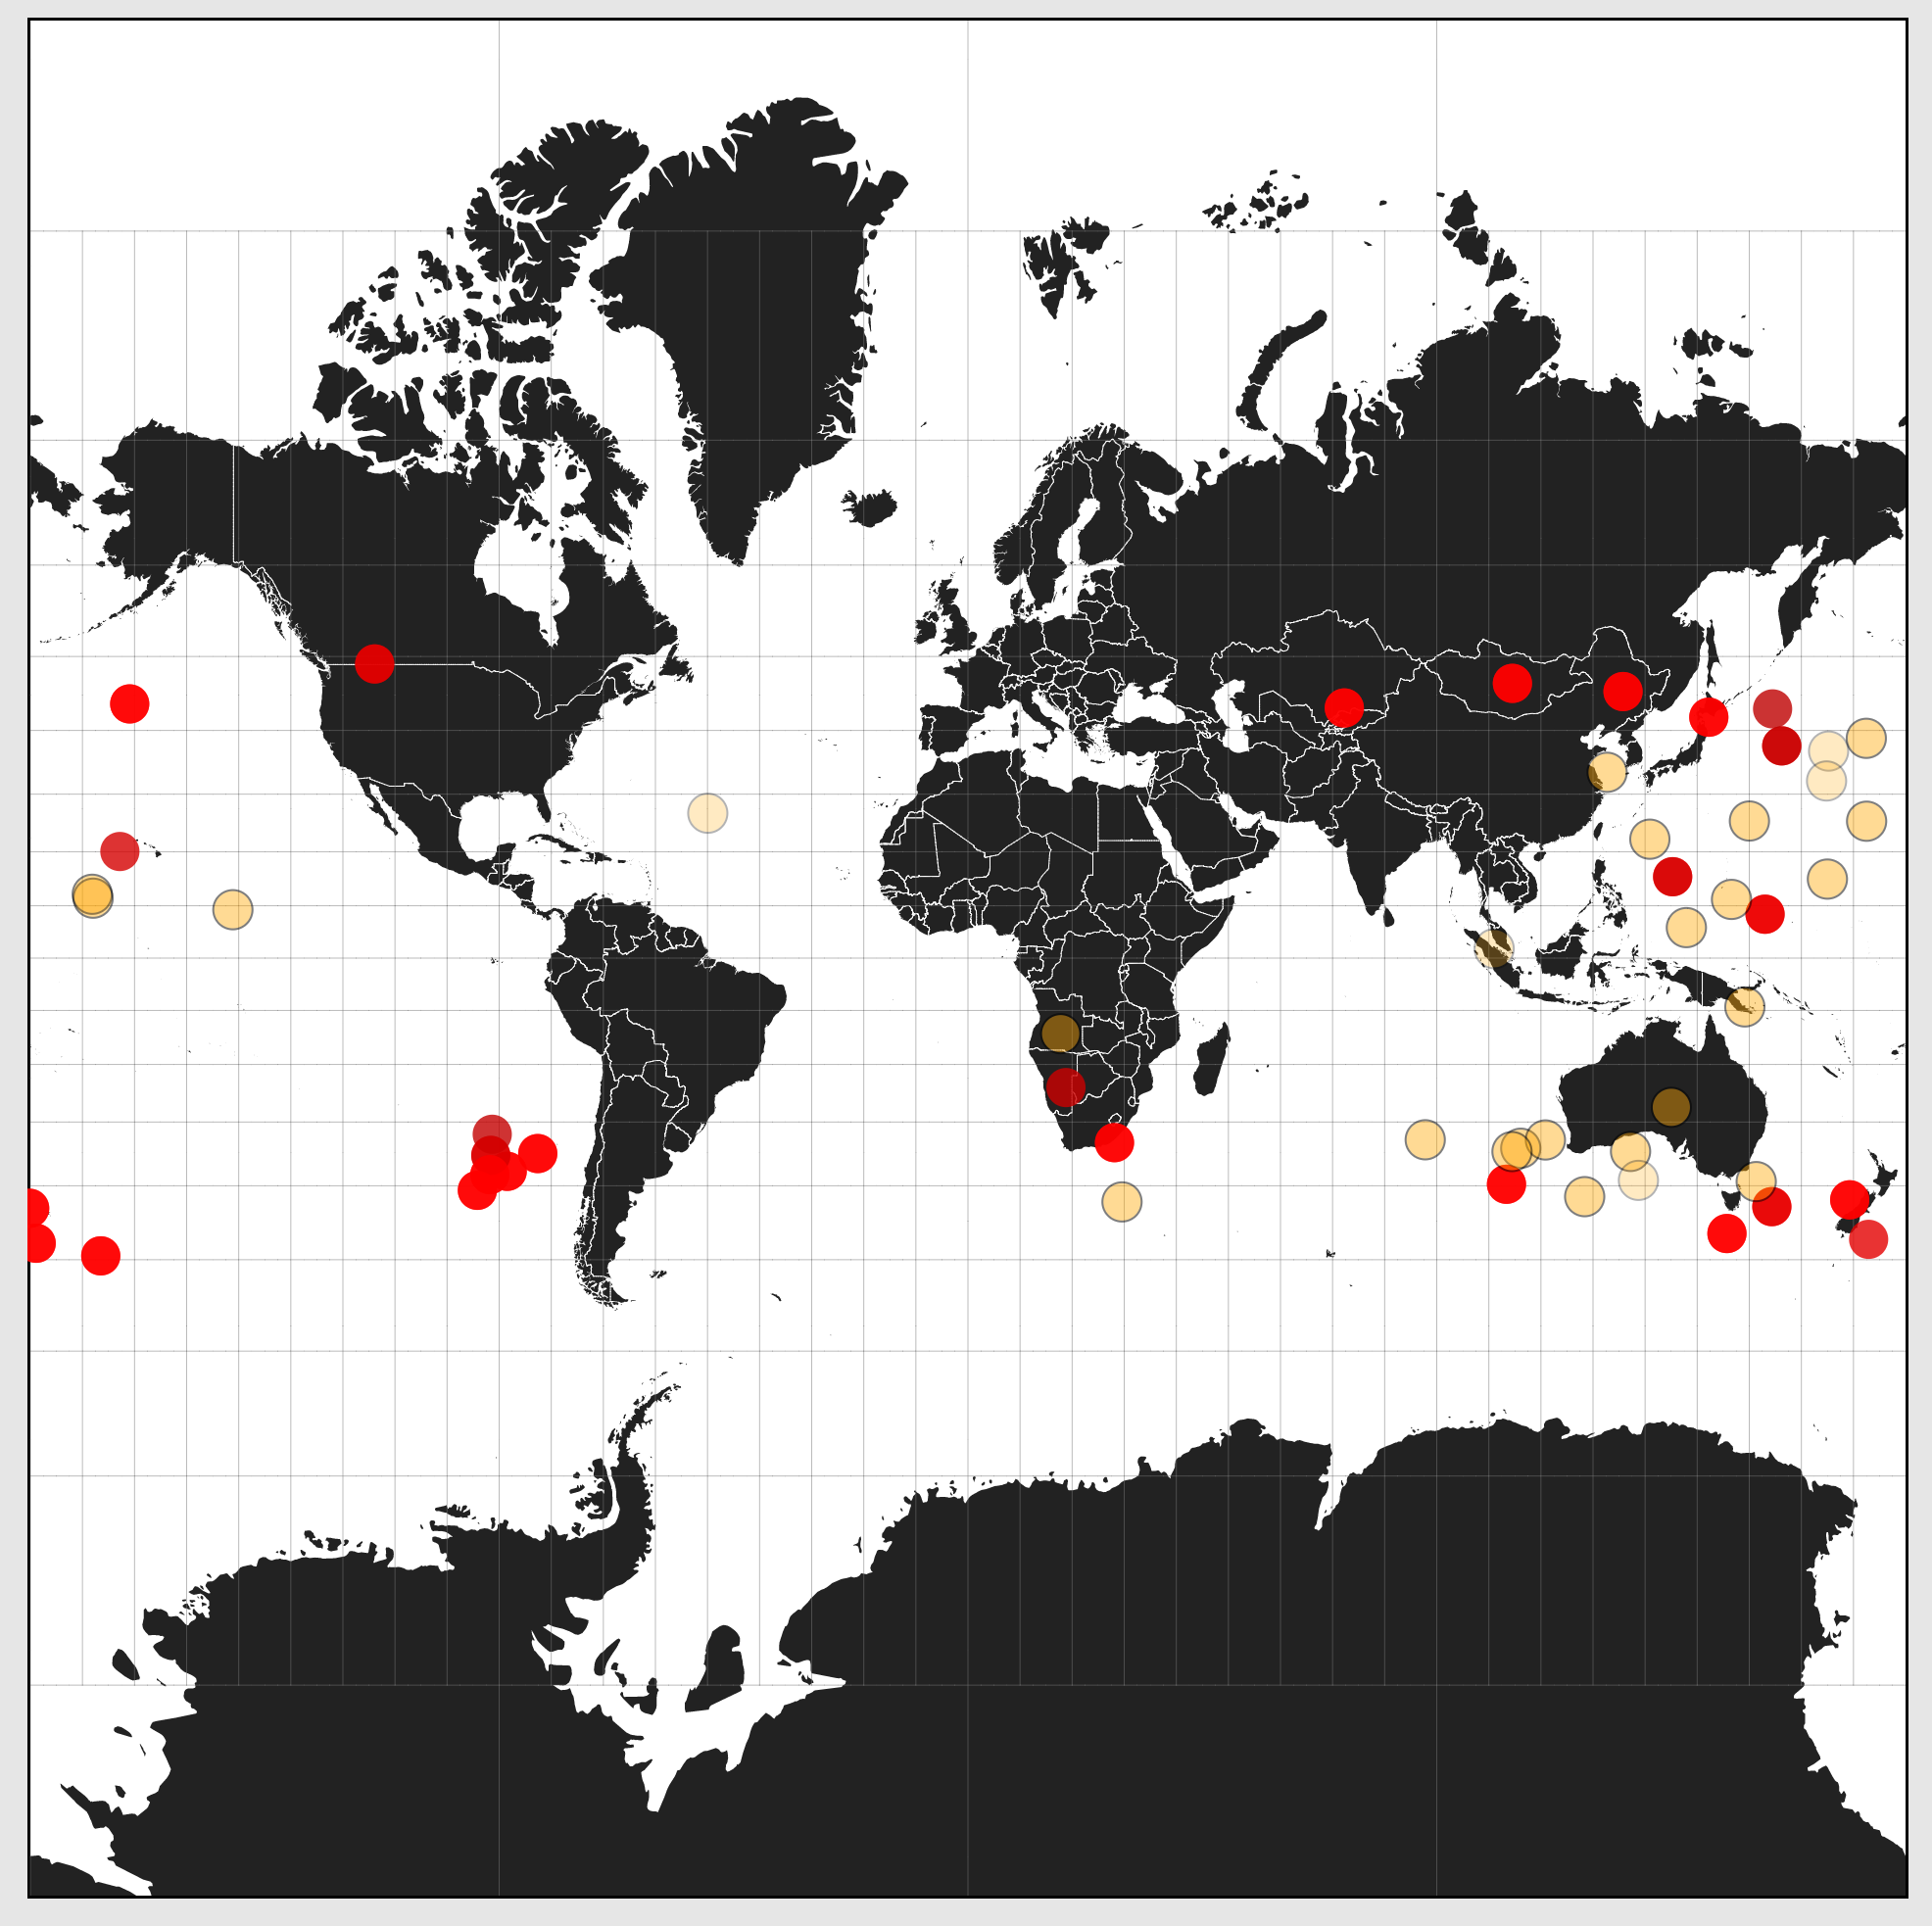
\includegraphics[width=\textwidth]{lat-long.png}
    \caption{Datapoints with darkrates above 4.5e-6, in native coordinates.  No strong grouping is observed.}
  \end{minipage}
  \hfill
  \begin{minipage}[b]{0.4\textwidth}
    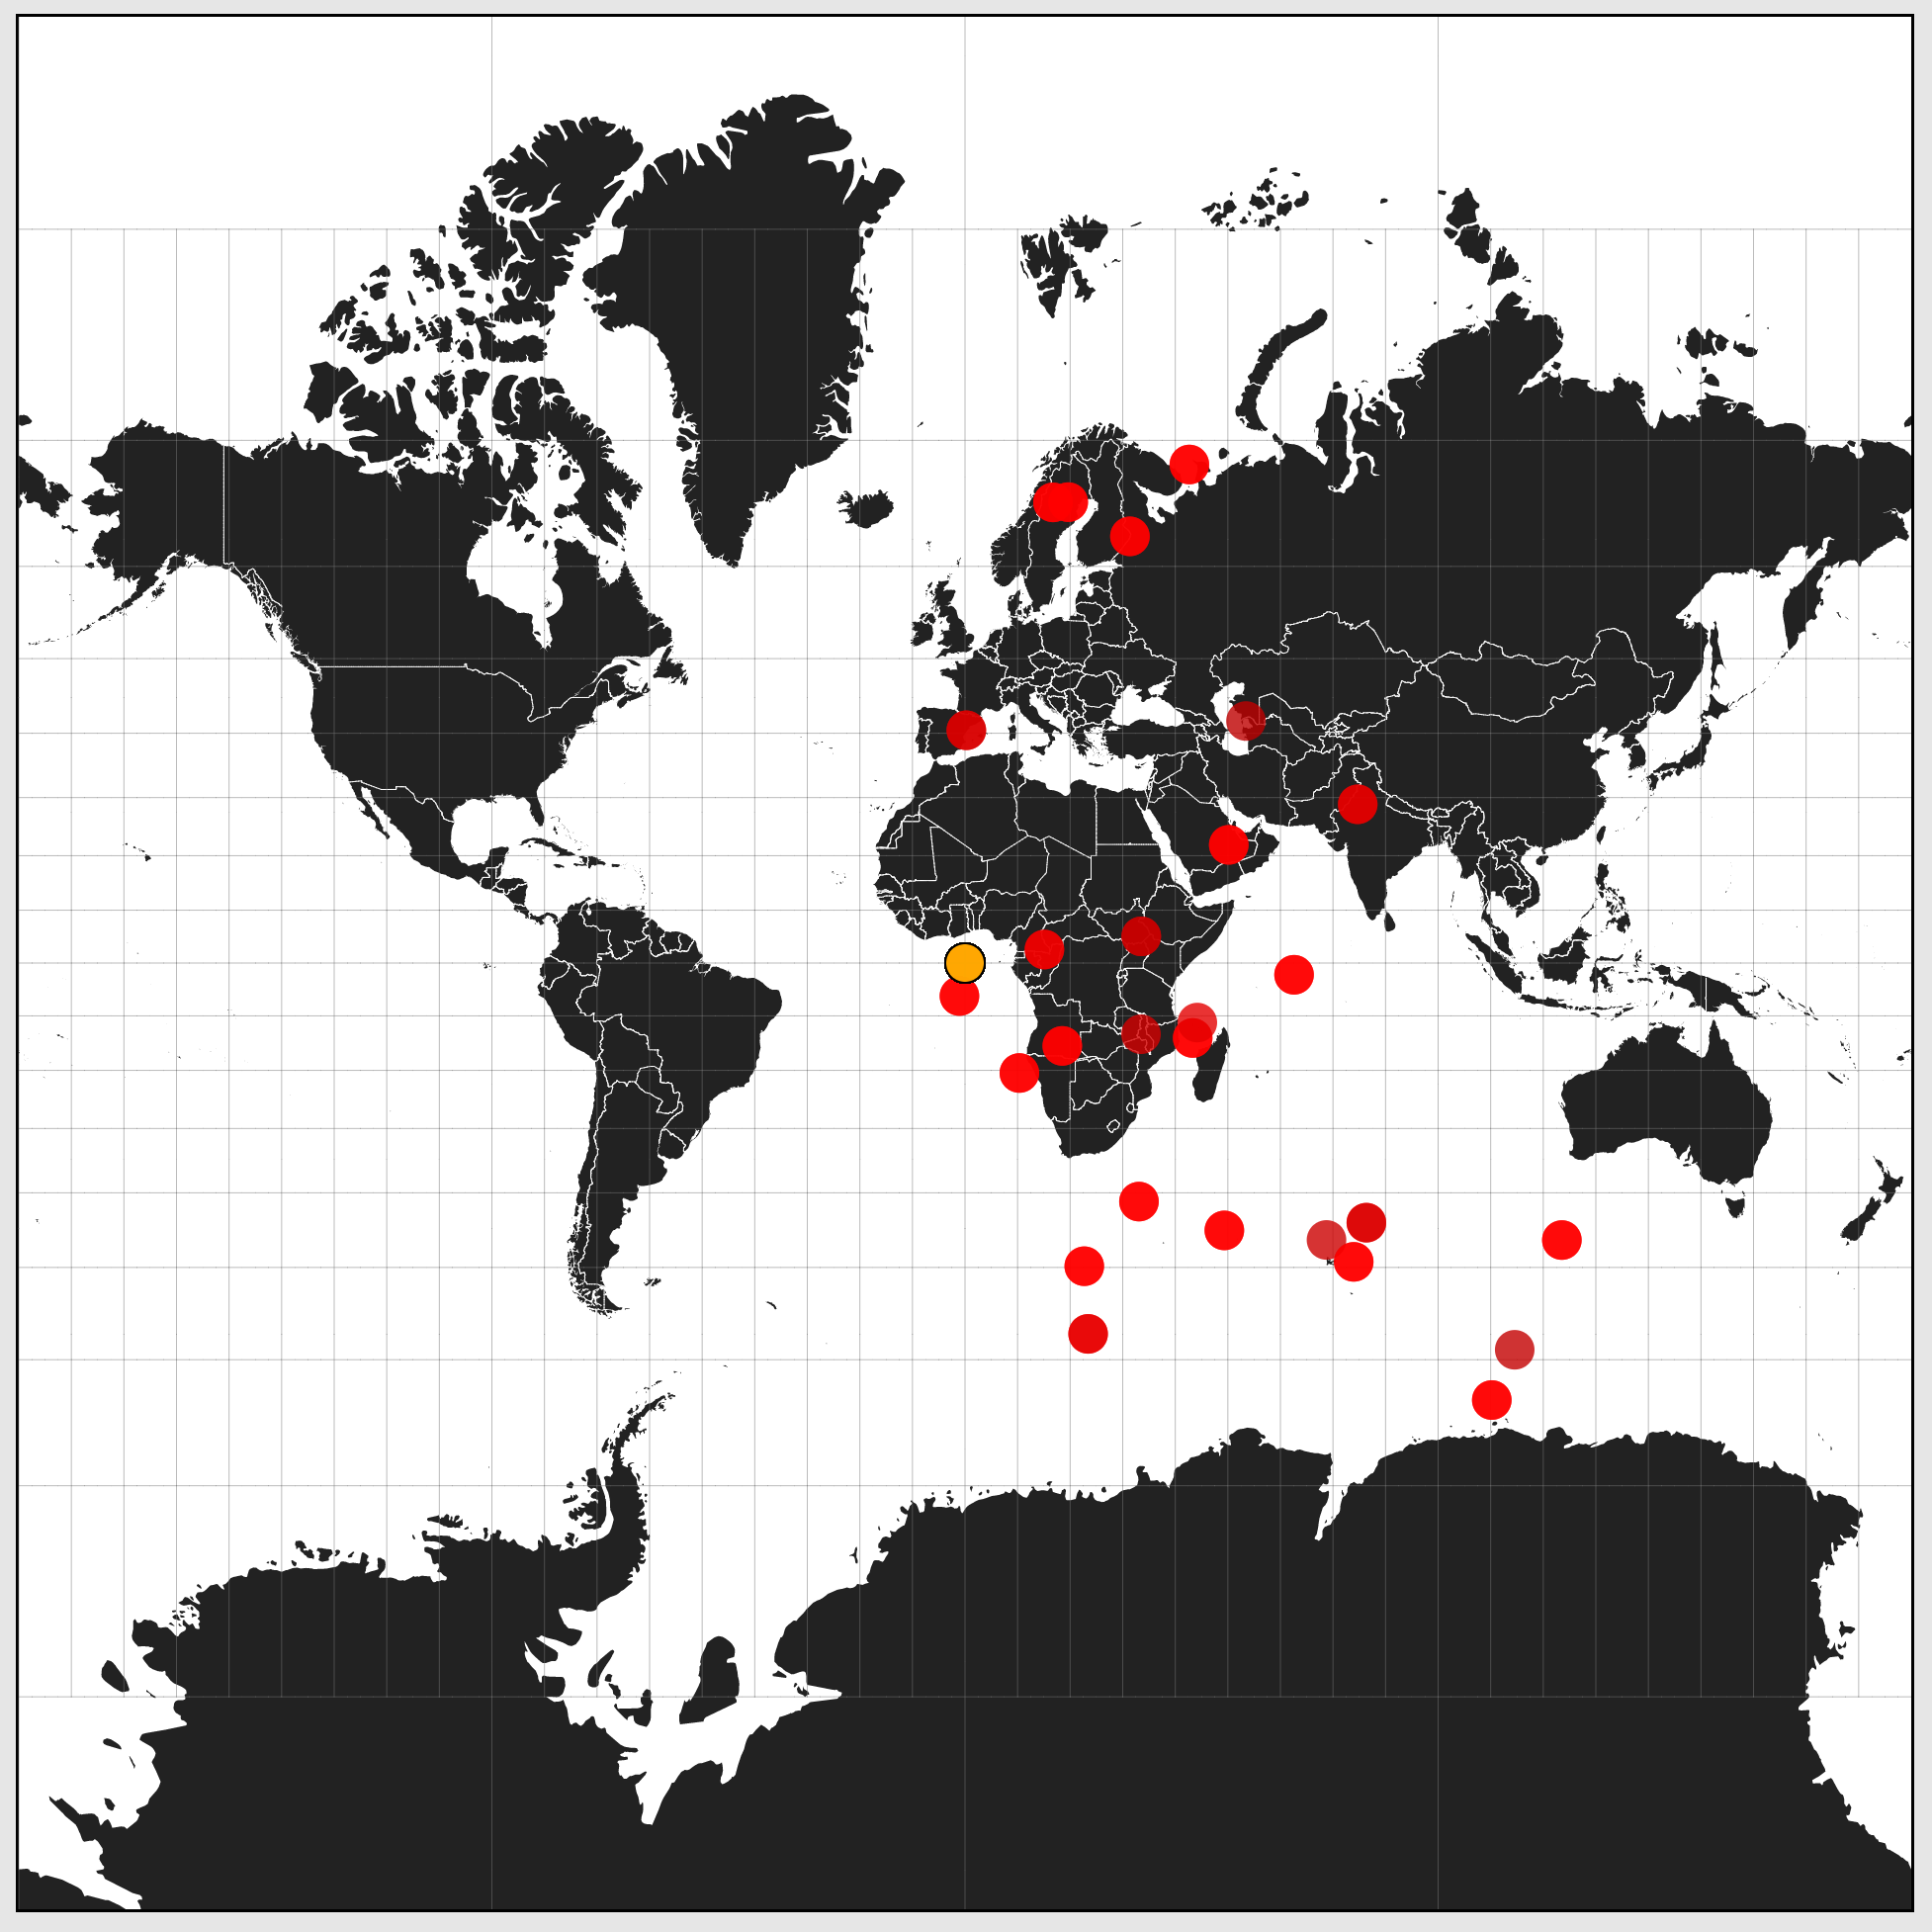
\includegraphics[width=\textwidth]{sub-solar.png}
    \caption{Datapoints with darkrates above 4.5e-6, relative to sub-solar point.  Strong grouping east of sub-solar is 
    well-pronounced.}
  \end{minipage}
\end{figure}


\section{Conclusion}
From this investigation, we find that significant darkrate spikes are well correlated with times when the HST orbital path crossed
a region east of the sub-solar point during periods of high solar output.  This matches well with a scenario in which 
the solar output of particles with UV and higher energies increases during the peak of the solar cycle.  These 
particles then travel the earth-sun distance and cross near the vicinity of HST's current position, slightly east of sub-solar due to the Earth's rotation.





\pagebreak



\begin{thebibliography}{9}
\bibitem{badhwar}
Badhwar, Gautam D.
\textit{The Radiation Environment in Low-Earth Orbit}. Radiation Research, vol. 148, no. 5, 1997, pp. S3–S10., www.jstor.org/stable/3579710.

\bibitem{fox}
Fox A. 
\textit{Cosmic Origins Spectrograph Instrument Handbook For Cycle 25}. Baltimore: Space Telescope Science Institute; 2017. Available at: http://www.stsci.edu/hst/cos/documents/handbooks/current/cos\_ihb.pdf. 

\bibitem{norton}
James B, Norton O, Alexander M. 
\textit{The Natural Space Environment: Effects On Spacecraft}. Washington, D. C.: NASA Marshall Space Flight Center; 1994. Available at: https://ntrs.nasa.gov/search.jsp?R=19950019455

\bibitem{lawrence}
Murr, Lawrence E., and William H. Kinard. 
\textit{Effects of Low Earth Orbit.} American Scientist, vol. 81, no. 2, 1993, pp. 152–165., www.jstor.org/stable/29774871.

\bibitem{mercedes}
Richards, Mercedes T., et al. 
\textit{Long-Term Variability in the Length of the Solar Cycle}.
 Publications of the Astronomical Society of the Pacific, vol. 121, no. 881, 2009, pp. 797–809., www.jstor.org/stable/10.1086/604667.

\bibitem{hst}
Wikipedia contributors. \textit{Hubble Space Telescope.} Wikipedia, The Free Encyclopedia. Wikipedia, The Free Encyclopedia, 7 May. 2017. Web. 9 May. 2017.

\bibitem{leo}
Wikipedia contributors. \textit{Low Earth orbit.} Wikipedia, The Free Encyclopedia. Wikipedia, The Free Encyclopedia, 7 May. 2017. Web. 9 May. 2017.



\end{thebibliography}

\pagebreak

\appendix
\section{Web Dashboard}
The active exploratory website can be found at \href{https://justincely.github.io/hstcos\_darkrates/}{https://justincely.github.io/hstcos\_darkrates/}.

\section{Data and Reduction Software Locations}

\begin{itemize}
	\item \href{https://github.com/justincely/calcos/tree/subsolarlink}{Custom calibration pipeline.}
	\item \href{https://github.com/justincely/hstcos\_dark\_data.git}{Dataset preparation.}
	\item \href{https://github.com/justincely/hstcos\_darkrates.git}{Webpage source code.}
\end{itemize}

%%%%%%%%%%%%%%%%%%%%%%%%%%%%%%%%%%%%%%%%%%%%%%%%%%%%%%%%%%


\end{document}
